\documentclass{beamer}
\usetheme{Boadilla}

\usepackage[english,greek]{babel}
% \usepackage[greek,english]{babel}
\usepackage[utf8]{inputenc}


\newcommand{\tl}{\textlatin}
\newcommand{\en}{\selectlanguage{english}}
\newcommand{\gr}{\selectlanguage{greek}}


% gia na mou vgazei ton titlo kathe fora
\AtBeginSection[]{
  \begin{frame}
  \vfill
  \centering
  \begin{beamercolorbox}[sep=8pt,center,shadow=true,rounded=true]{title}
    \usebeamerfont{title}\insertsectionhead\par%
  \end{beamercolorbox}
  \vfill
  \end{frame}
}
\usepackage{xmpmulti}

\usepackage{tikz}   

\graphicspath{ {./pictures/} }       % path for images
\title{Αναγνώριση και εντοπισμός ανθρώπινης δραστηριότητας σε βίντεο}
\author{Στάθης Γαλανάκης}
\date{\today}

\begin{document}
\gr
\begin{frame}
\titlepage
\end{frame}


\begin{frame}
  \frametitle{\tl{Outline}}
  \tableofcontents[pausesections]
\end{frame}


% \documentclass{beamer}
% \usetheme{Boadilla}

% \usepackage[english,greek]{babel}
% % \usepackage[greek,english]{babel}
% \usepackage[utf8]{inputenc}

% \newcommand{\tl}{\textlatin}
% \newcommand{\en}{\selectlanguage{english}}
% \newcommand{\gr}{\selectlanguage{greek}}


% \begin{document}

\section{Εισαγωγή}

\begin{frame}
  \frametitle{Περιγραφή προβλήματος}
  Το πρόβλημα της αναγνώρισης και εντοπισμού ανθρώπινης δράσης σε βίντεο έχει δύο κύριους στόχους:
  \begin{itemize}[(I)]
  \item<2-> Την αυτόματη αναγνώριση και ταξινόμησή οποιασδήποτε ανθρώπινης δραστηριότητας στο βίντεο.
  \item<3-> Τον αυτόματο εντοπισμό αυτής της δράσης στο βίντεο
  \end{itemize}

\end{frame}

\begin{frame}
  \frametitle{Προκλήσεις και \tl{Datasets}}
  \begin{figure}
    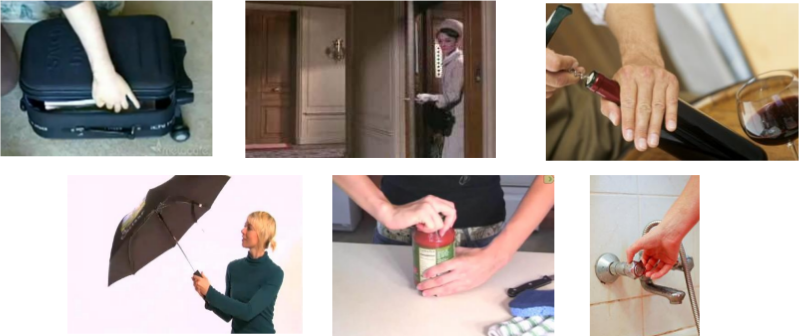
\includegraphics[scale=0.2]{open_example}
  \end{figure}
  \pause
  Παραδείγματα της δράσης «Ανοίγω»

\end{frame}




% \subsection{Applications}
% \subsection{Challenges and Datasets}
% \subsection{Motivation and Contributions}
% \end{document}
% \documentclass{beamer}
% \usetheme{Boadilla}

% \title{Thesis}
% \subtitle{Action Recognition and Localization}
% \author{Stathis Galanakis}
% \institute{National University of Athens}
% \date{\today}

% \begin{document}

\section{Tube Proposal Network}

\subsection{Approach 1}
\subsection{Approach 2}

% \end{document}
% \documentclass{beamer}
% \usetheme{Boadilla}

% \title{Thesis}
% \subtitle{Action Recognition and Localization}
% \author{Stathis Galanakis}
% \institute{National University of Athens}
% \date{\today}

% \begin{document}

\section{Connection Algorithm}

\subsection{Approach 1}
\subsection{Approach 2}
\subsection{Approach 3}
% \end{document}

\section{Classification stage}

% \subsection{First results}
\begin{frame}
  \frametitle{First}
\end{frame}
% \subsection{Adding more groundtruth tubes}
% \subsection{MLP}
% \subsection{Adding NMS algorithm}
% \end{document}

\end{document}